\chapter{The Completed Application}

As of the time of writing, Aphantasia is a functional proof of concept with a simple UI, graph view, and several rudimentary features.
While there are bugs to resolve and features to add, the application is usable and publicly accessible.

We are hosting two public instances:
\begin{itemize}
\item English version at \href{https://aphantasia.io}{aphantasia.io}
\item Czech version at \href{https://afantazie.cz}{afantazie.cz}
\end{itemize}

\section{Features}
This section provides a deeper look into the user-facing features and technical aspects of the application.
More user-focused documentation will be available in Chapter 6.

\subsection{AuthX/Y}
The application includes user account functionality, supporting authentication and authorization.
Users can register, log in, and log out. Most pages and features are accessible only to logged-in users.

Passwords are hashed using \gls{sha256} encryption and must meet minimal requirements:
\begin{itemize}
\item At least 8 characters
\item At least one uppercase letter
\item At least one lowercase letter
\item At least one number
\end{itemize}

Login is managed via \gls{jwt} stored in \gls{local_storage}.
Tokens expire after one day, and a refresh token mechanism is not implemented, requiring users to re-login every 24 hours.

Tokens are currently sent in URL parameters for SignalR WebSocket connections.
This practice is not ideal and should be replaced in the future.
A possible solution involves a ticketing system where a logged-in client would request a ticket from the API.
This ticket would then authorize the WebSocket connection, avoiding token exposure in the URL. %\xxx{cit?}

\subsection{Pages}
Thanks to React, the graph view is one of many pages in the application. There are currently ten pages:
\begin{itemize}
\item \textbf{Homepage}: Displays a feed of recent thoughts and navigation buttons (Figure \ref{obr:afantazie_welcome_and_homepage})
\item \textbf{Welcome Page}: Similar to the homepage but tailored for unregistered users (Figure \ref{obr:afantazie_welcome_and_homepage})
\item \textbf{About Page}: Provides information about the project
\item \textbf{Chat Room}: A basic real-time chat
\item \textbf{Settings Page}: Contains user settings and a logout button
\item \textbf{Login and Registration Pages}
\item \textbf{Notifications Page}: Displays replies from other users
\item \textbf{Graph View}: Enables users to view thoughts
\item \textbf{Thought Creation Page}: Allows users to create new thoughts
\end{itemize}

\begin{figure}[p]
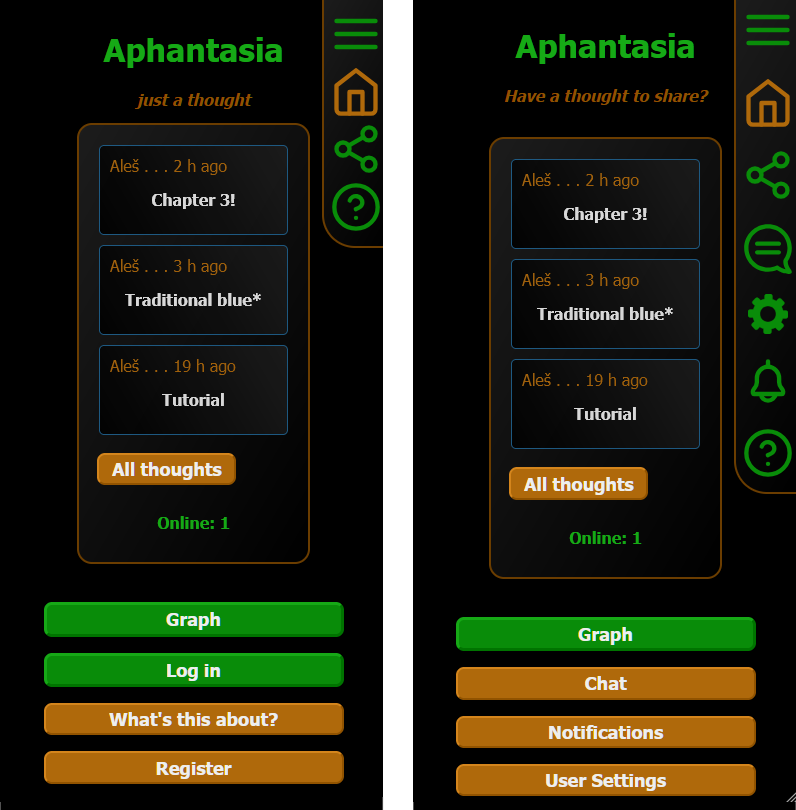
\includegraphics[width=130mm, keepaspectratio]{img/afantazie_welcome_and_home_page.png}
\caption{The Welcome page and homepage of Aphantasia}
\label{obr:afantazie_welcome_and_homepage}
\end{figure}

\subsection{Localization}
Initially, we developed a Czech version of the application and later added an English version.
For frontend \gls{localization}, we utilized two JSON files and a Localization object which returns 
either czech or english text based on \gls{vite} configuration.
This makes the application easily extensible to more languages.

Backend localization was also required, as the API returns localized authentication and validation messages.
To achieve this, we created a Localization project with classes implementing localization interfaces.
During boostrapping a specific localization is registered based on configuration. 
While this approach is somewhat cumbersome, it suffices for the limited localization needs of the backend.

\subsection{Custom Graph Rendering Engine}

The graph view is the primary feature of Aphantasia and the most complex part of the application.
Its basic features include:
\begin{itemize}
\item \textbf{Zooming and Panning}
\item \textbf{Dragging Thoughts}
\item \textbf{Floating Text Titles} (figure \ref{obr:afantazie_floating_titles})
\item \textbf{Thought Highlighting} (On figures \ref{obr:afantazie_mobile_graph_view} and \ref{obr:afantazie_floating_titles})
\end{itemize}

\begin{figure}[p]
    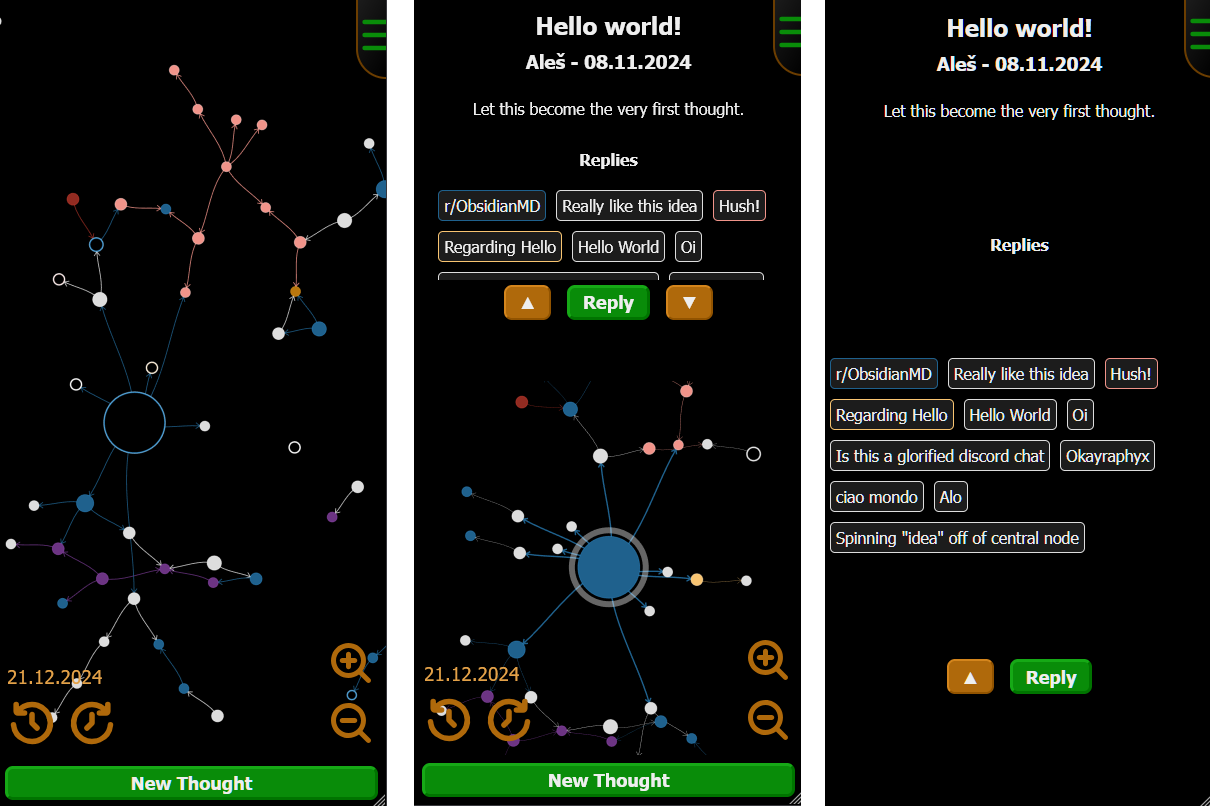
\includegraphics[width=130mm, keepaspectratio]{img/afantazie_mobile_graph_view.png}
    \caption{The graph view on mobile device - non-highlighted mode, half-screen preview and fullscreen preview respectively}
    \label{obr:afantazie_mobile_graph_view}
\end{figure}


\begin{figure}[p]
    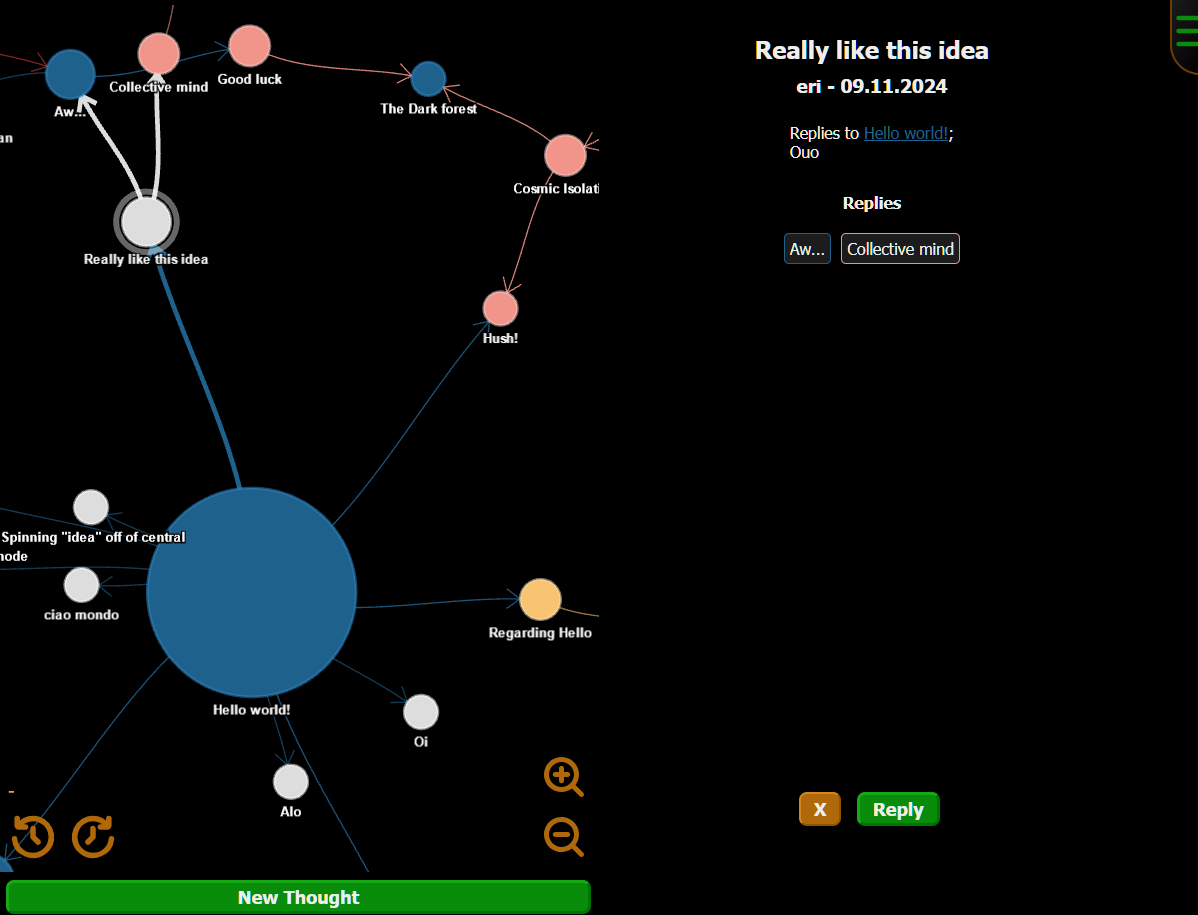
\includegraphics[width=130mm, keepaspectratio]{img/afantazie_floating_titles.png}
    \caption{Floating titles in the graph view on desktop}
    \label{obr:afantazie_floating_titles}
\end{figure}

% The graph view utilizes Pixi.js for rendering, \gls{zustand} for state management, and a custom \gls{FDL} implementation.
% move to implementation- todo

We began with pull and push forces and incrementally introduced a range of parameterizable settings to the computation.
\begin{itemize}
\item \textbf{Forces}: Pull force, push force, and gravity force, including maximum allowed values and distance thresholds
\item \textbf{Link Distance}: Controls the spacing between connected thoughts
\item \textbf{Momentum Dampening Divisor}: Forces acting on thoughts are divided by this number resulting in a smoother less shaky simumeaning lation
\item \textbf{Stage Size}: The size of the simulation container
\item \textbf{Radius Controls}: Base radius, size multiplier (how much larger more-referenced thoughts are) and maximum radius
\item \textbf{Simulation Falloff Time}: Gradually slows down the \gls{GLA} after each user interaction (dragging, or selecting thoughts and time sliding)
\item \textbf{Frames with Overlap}: Allows newly appeared thoughts to overlap for given amount of frames
\item \textbf{Layout Caching Frequency}: Specifies how often the layout is saved to \gls{local_storage}
\item \textbf{Node Mass}: Allows differently sized thoughts to have proportional influence on each other, with maximum and minimum values also parametrized
\item \textbf{Backlinks Count Force Divisor}: Reduces forces acting on highly connected nodes
\item \textbf{Edges Appearance}: Adjusts thickness and color of highlighted and unhighlighted edges (edges leading in or out of the currently highlighted node)
\item \textbf{Frames with Less Influence}: New thoughts start with no influence over the simulation and gradually gain it over time
\end{itemize}

This is a non-exhaustive list and there are many more parameters controlling the simulation and rendering process.

\begin{figure}[p]
    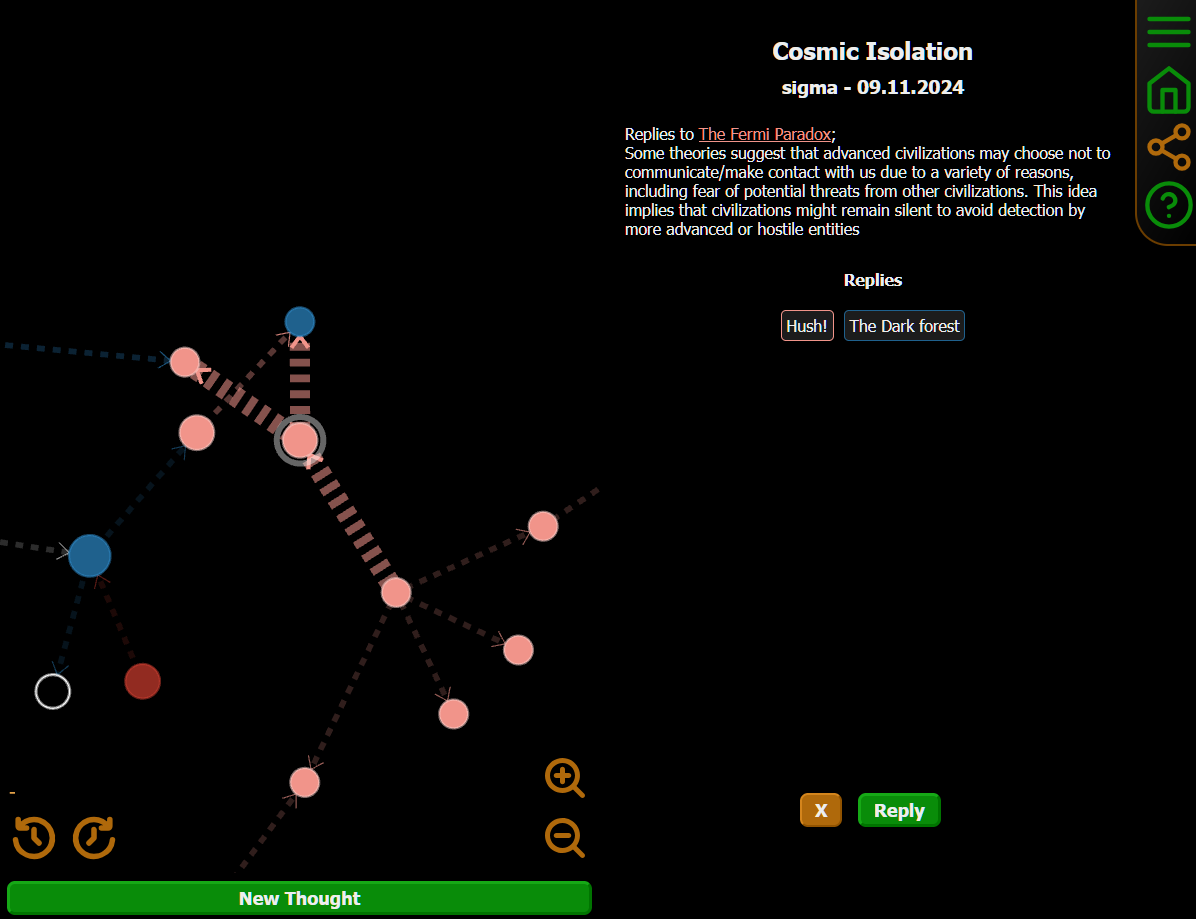
\includegraphics[width=130mm, keepaspectratio]{img/afantazie_animated_edges.png}
    \caption{Animated edges in the graph view}
    \label{obr:afantazie_animated_edges}
\end{figure}
    
\subsubsection*{On-screen thoughts limit}
The On-screen thoughts limit is a critical part of our big graph rendering solution.
The default value is 100, but users can adjust it in the settings.

The idea behind it is to always render at most this number of thoughts on screen.
And to view more user input is required - either by moving the time slider or by using the Graph walk feature, both of which we will talk about briefly.

The limit is demonstrated in figures \ref{obr:afantazie_production_dataset_in_time_window} and \ref{obr:afantzazie_production_dataset_640_nodes} with the values set to 300 and 700 respectively.

\subsubsection*{Time Slider}
Combining the On-screen thoughts limit, dynamic loading, and two UI buttons resulted in a feature we call the Time slider.
It allows users to move a conceptual time window smoothly into the past or future by holding the corresponding button.
The resulting layout using time slider is demonstrated in figure \ref{obr:afantazie_production_dataset_in_time_window}
with 641 thoughts on afantazie.cz viewed in three different time windows of length 300.

Above the time slider controls there is a label showing the current time window's position - the creation date of the newest thought on screen.
You can see the label in bottom left in figure \ref{obr:afantazie_mobile_graph_view}.

New thoughts appear either in their cached positions (see Layout caching section below) or in a circular pattern around the simulation container’s center.
When not yet cached the appearance of newer/older nodes creates a visually appealing effect as the thoughts gradually appear in what resembles a loading spinner.

\subsubsection*{Live Preview}
When the time slider moves beyond the last thought, the application enters live preview mode indicated by 'Now...' apearing in place of the time window's date in bottom left.
In this mode the client listens for new thoughts and adds them to the graph in real time.

While this feature enhances interactivity, it has only been tested with two users creating thoughts simultaneously.
Higher activity levels could potentially overwhelm the interface but until there is an active userbase this remains a theoretical concern.

\subsubsection*{Graph Walk}
The neighborhood API endpoint powers Graph walk demonstrated in figure \ref{obr:afantazie_mobile_graph_view}.
After clicking on a node, link or reply the client loads the neighborhood of the newly highlighted thought, enabling interactive exploration.

In the example as well as many other screenshots provided in this work, some thoughts appear hollowed out.
This effect triggers when thought's direct neighbors (links or replies) are not currently rendered on screen
signalling that there is more to explore behind it.
When the neighbors of a node are all visible, the node is filled with its author's color.

Currently graph walk doesn't respect the on-screen thoughts limit and loads all neighbors of the highlighted thought up to given depth. This didn't pose a problem with the datasets we used but could be a significant issue with highly connected datasets.

\subsubsection*{Thoughts Layout Caching}
The browser’s local storage caches the thoughts layout after a period of inactivity.
The length of this period is parametrizable by number of frames,
with the current value set to 1000 frames which corresponds to around 30 seconds of inactivity on most devices.
When a thought leaves the screen and later reappears, it retains its previous position.
This feature facilitates graph stability during time sliding and between sessions and removes the need for the graph to re-stabilize again and again.

Paired with the Time slider this approach produced an unexpected emergent behavior. As the \gls{production} dataset grew beyond 500 thoughts (five times the default on-screen limit), it remained possible to create a stabilized graph across the entire dataset.
Moving the time slider across such stabilized layout is a uniquely satisfying experience, which we believe sets Aphantasia apart.
To some extent, this feature is visible in figure \ref{obr:afantazie_production_dataset_in_time_window} but it is best experienced in the live application.

The cache currently has no size limit and is not cleared automatically, which could be a potential issue with big datasets and longer graph view sessions.
Logged in users can however delete cached positions in settings to force the graph to re-stabilize.

\begin{figure}[p]
    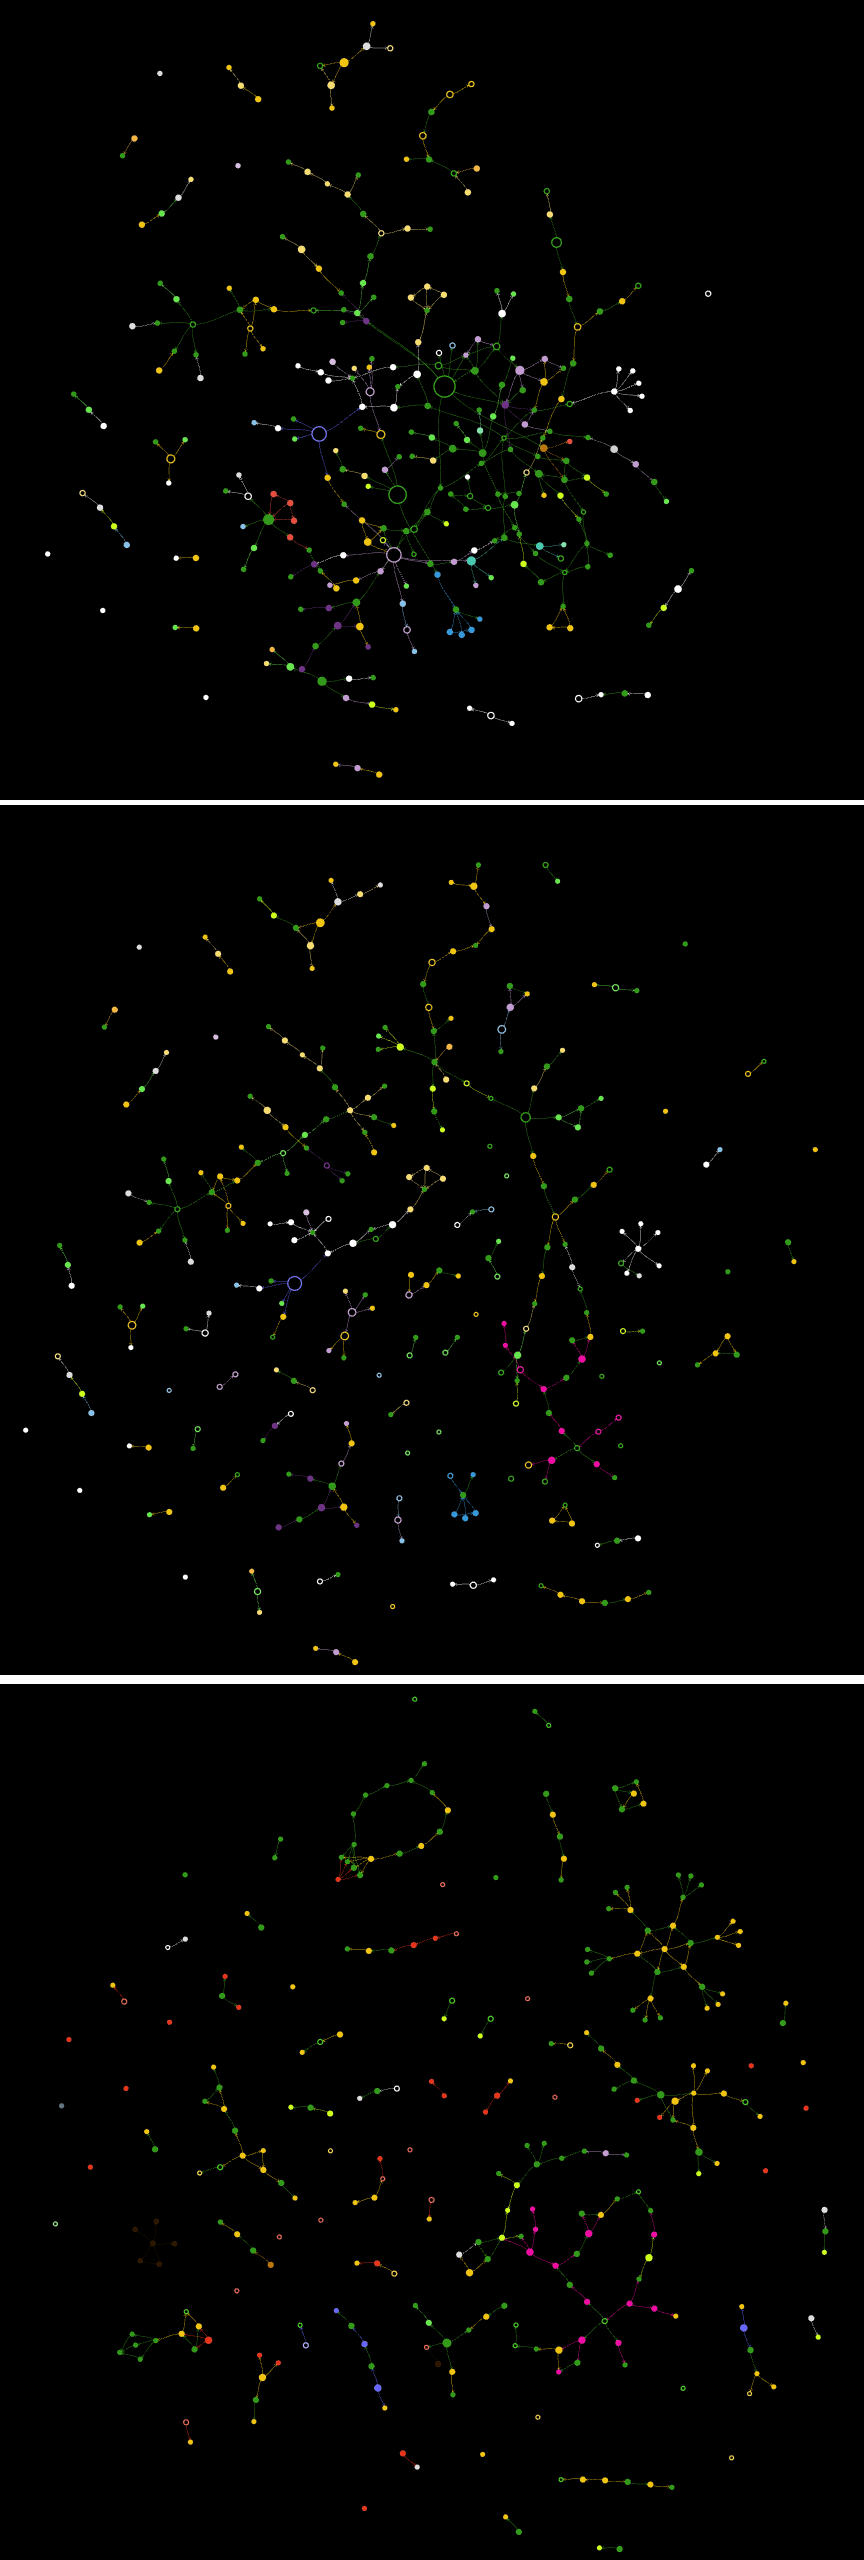
\includegraphics[height=200mm, keepaspectratio]{img/afantazie_production_dataset_in_time_window.png}
    \caption{Aphantasia with the czech production dataset in stabilized temporal layout (641 nodes in three time windows of length 300)}
    \label{obr:afantazie_production_dataset_in_time_window}
\end{figure}

\begin{figure}[p]
    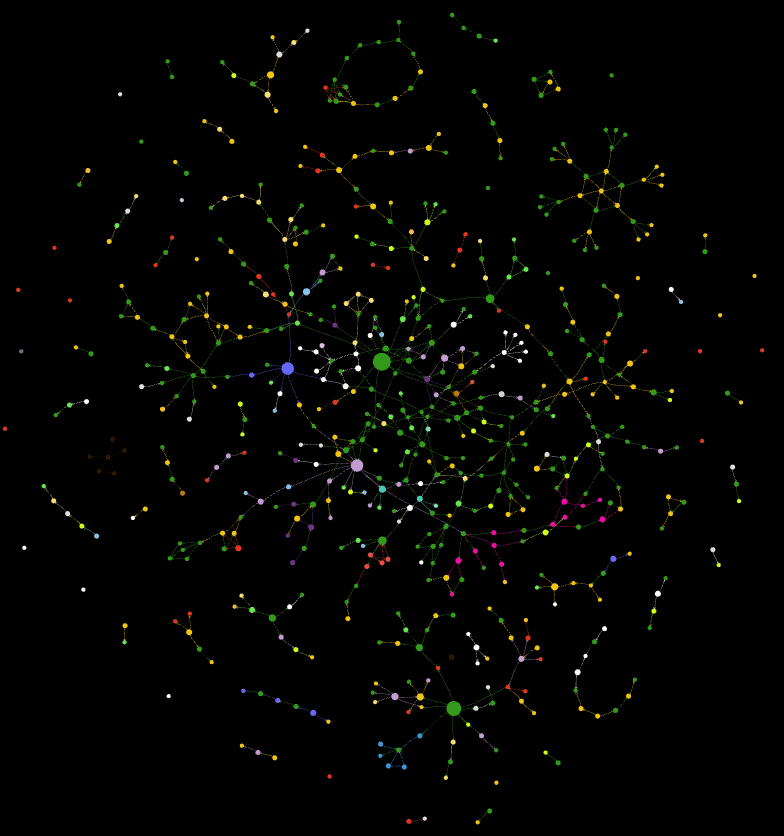
\includegraphics[width=130mm, keepaspectratio]{img/afantzazie_production_dataset_641_nodes.png}
    \caption{The entire dataset of afantazie.cz (641 nodes) in a single time window}
    \label{obr:afantzazie_production_dataset_640_nodes}
\end{figure}

\subsubsection{Animated edges}
This feature is currently unused and unparametrized (instead it is just commented out in the source code) but is worth mentioning.
Instead of the curved arrows used by default these edges consist of a series of sections flowing from referenced thought to its replies. This helps to visualize the flow of time from older to newer posts.

You can see screenshot of this feature in figure \ref{obr:afantazie_animated_edges}.
It remains unused as the animation has small visual artifacts but once fixed could be added as an optional setting.

\section{Graph View Performance}

The graph can handle the entire CitHep dataset and thanks to dynamic loading could handle even larger graphs.
On figure \ref{obr:afantazie_cithep_highlighted_thought} you can see a highlighted thought from the \gls{cithep_dataset} dataset.

To achieve this we wrote a C\# script to import the CitHep data files into Aphantasia database.
In graph view we used the same parameter settings we used for the much smaller graphs in \gls{production} environment
which at the time consisted of around 600 and 150 thoughts respectively.
To our surprise the resulting graph behaved well and except for increased tendency to jitter the CitHep graph view was smooth and stable.
The only parameter we had to change was neighborhood \gls{BFS} depth - from three down to just one.
CitHep graph is bigger and much more interconnected than the small production graphs so even at depth two
the graph walk feature often resulted in unreasonable amount of on-screen nodes.

\subsection{Limits of the Graph View}

In the previous chapter, in figure \ref{obr:afantazie_cithep_3k}, we have seen how Aphantasia handles 3000 nodes. 

The application is not meant to display large graphs at once, but out of curiosity we tried to render as many thoughts as possible.

First we tried to set the on-screen thought limit to 40000 (and thus load and render the entire CitHep dataset) and we were not able to fetch the data from the backend.
We are not sure why this happened but one possible explanation is that the API response is too large and either the server and/or the client were not able to handle it.

In the second test we set the on-screen thought limit to 10000 and we were able to fetch the data and render it.
The result was not unexpected - a big hairball of nodes and edges running at less than 1 frame per second.
See figure \ref{obr:afantazie_cithep_10000_on-screen-limit}.


\begin{figure}[p]
    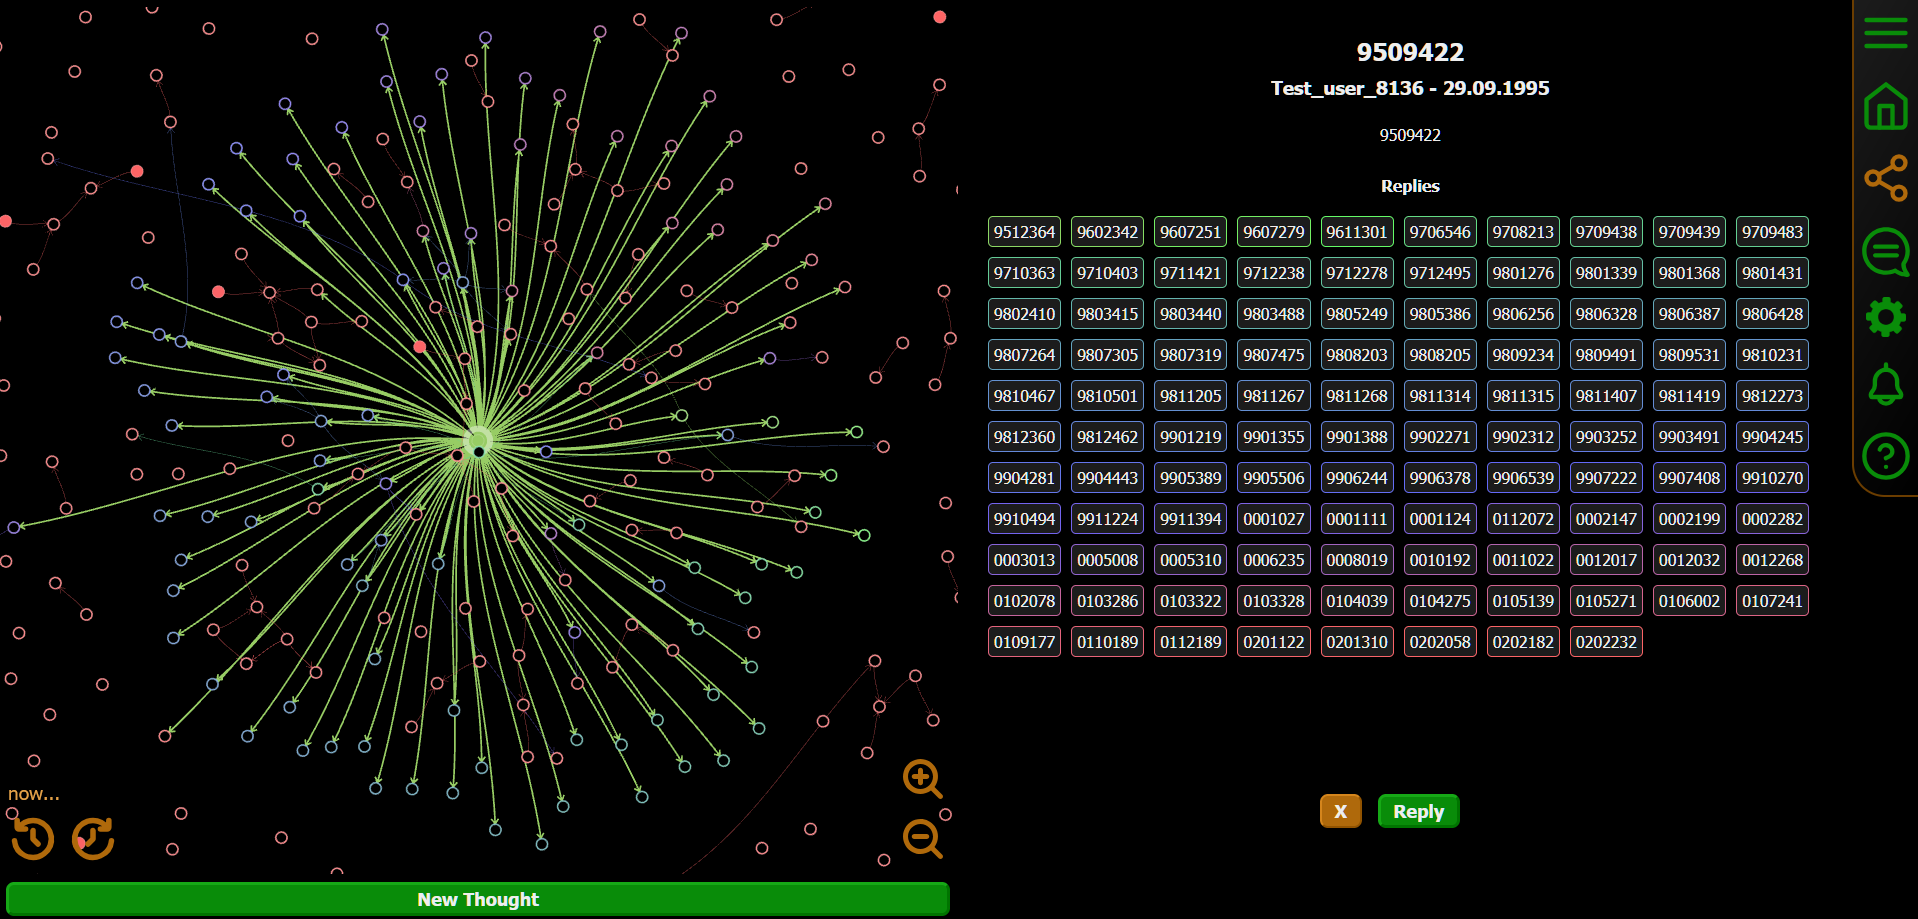
\includegraphics[width=130mm, keepaspectratio]{img/afantazie_cithep_highlighted_thought.png}
    \caption{A highlighted thought of the CitHep Dataset in Aphantasia}
    \label{obr:afantazie_cithep_highlighted_thought}
\end{figure}

\begin{figure}[p]
    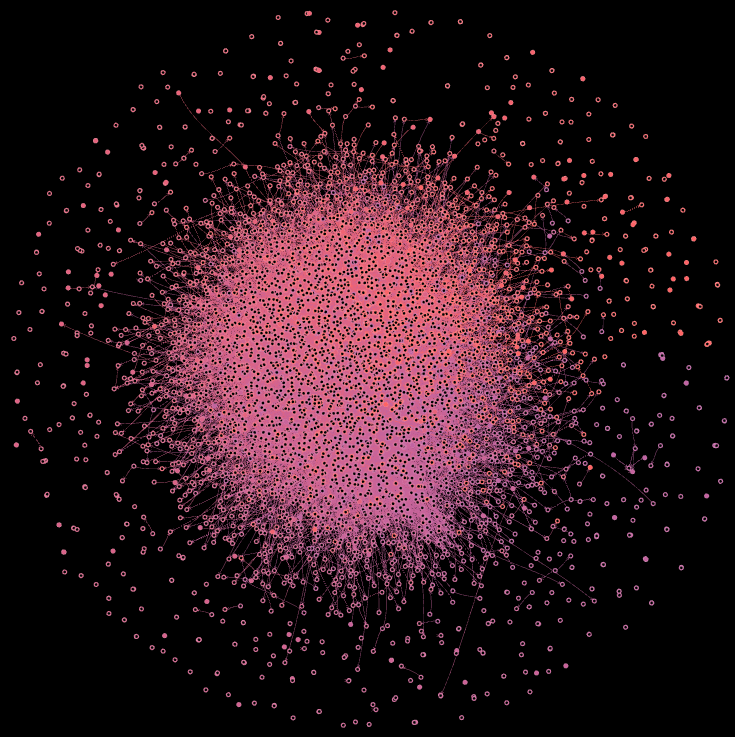
\includegraphics[width=130mm, keepaspectratio]{img/afantazie_cithep_10000_on-screen-limit.png}
    \caption{Cithep dataset rendered in Aphantasia with 10000 on-screen thought limit}
    \label{obr:afantazie_cithep_10000_on-screen-limit}
\end{figure}

From our tests we learned that Aphantasia's performance begins to degrade noticeably at around 400-700 on-screen thoughts limit and gradually drops to just few frames per second with the limit set to around 1,500.
These values are highly dependent on the connectivity of the data, with more connections leading to more computation time and thus lower performance.

\section{Deviation from the Original Plan}
Initially, we planned to implement a zoom-based dynamic loading and rendering system for large graphs.
However, we opted for a time-based and proximity-based approach (e.g., the time slider and neighborhood).

This decision was primarily driven by ease of implementation.
While zoom-based techniques remain valid, they are more complex and could have delayed progress.
The time slider naturally emerged as a consequence of the thoughts-on-screen limit, making zoom-based dynamic laoding a redundant feature to pursue further.

We also omitted filtering and searching functionalities.
These features are not critical, as graph exploration begins within a time window (latest or around a specific thought) and continues interactively.
The time saved was redirected to parameterizing and bug-fixing the graph view.
We still plan to implement these features in the future, as the architecture supports them and they will frther enhance the user experience.

\section{Future Development}

Although functional, Aphantasia remains an unpolished prototype.
Several significant issues and bugs require attention.
Some have already been mentioned in the previous sections, but the most pressing are:

\begin{itemize}
\item \textbf{Graph View Buttons}: Zoom and time slider controls often get stuck on mobile devices.
\item \textbf{Pinch Zoom}: This standard mobile feature is currently missing, making the graph view less intuitive on touch devices.
\item \textbf{Jitter}: While mostly resolved, occasional oscillations during node stabilization persist.
\item \textbf{Bugs}: Some notable issues include neighborhood thoughts persisting after graph view exit and re-entry. The Zustand graph store initialization needs an overhaul.
\item \textbf{Graph View Limits}: Neighborhood thoughts are not limited by the on-screen thoughts limit, thought positions cache has no size limit 
\item \textbf{Tutorial}: A tutorial is necessary to help new users understand the application, especially those unfamiliar with graph visualization.
\item \textbf{Backend Validation}: The backend’s Create Thought endpoint has a redundant links parameter, leading to potential inconsistencies when used programmatically.
\item \textbf{Notifications}: The current system lacks paging and cannot distinguish between read and unread notifications.
A dedicated notifications table could address these issues and enable more diverse notification types.
\end{itemize}

Despite these issues, Aphantasia has met and exceeded many of our expectations and the prototype stands on solid grounds, ready for further development.
After refining the prototype and fixing the problems, we plan to add new features and improvements, such as:
\begin{itemize}
\item Streamlining UI and UX
\item Filtering/Search
\item More graph algorithms besides \gls{FDL}
\item Email Verification
\item Password Reset functionality
\end{itemize}

\section{User Feedback}
We advertised the application on Reddit, sharing both the Czech and English versions across several subreddits.

Most comments were positive, praising the application’s concept and the experience of exploring thoughts
with one user describing the experience as feeling like an “archeologist” uncovering ideas. \xxx{cit?}

Negative feedback focused on the lack of practicality, outdated UI, and occasional bugs.
Users also suggested missing features such as pinch zoom, image posting, a better landing page, and filtering.
Browser compatibility issues were mentioned as well.

The feedback was mostly constructive and we are grateful for it.
It helped us hone on the experience users already found fun and stimulating, specifically interaction and exploration.
However, some users admitted they did not understand the application, highlighting the need for a proper tutorial.

\section{Aphantasia Versus Related Software}

Ideologically Aphantasia is closest to Obsidian.
There is of course an obvious difference between the two - Obsidian is local note-taking system with graph view while Aphantasia is an online social experience based on graph view.
Both are however meant for general audience and their graph views bare a similarity.

Compared to Gephi and Cytoscape.js Aphantasia has lower performance on large graphs rendered at once.
However thanks to Time slider and Graph walk features it can handle much larger datasets in an intuitive way.
The dynamic loading could in theory handle millions of nodes. In such case the main limiting factor would be the performance of the backend and the database.

Finally in table \ref{tab:comparison_2} we added Aphantasia to the comparison table from the first chapter.

\begin{table}[ht]
    \centering
    \caption{Comparison of Obsidian, Gephi, Cytoscape.js and Aphantasia}
    \label{tab:comparison_2}
    \begin{tabularx}{\textwidth}{|l|X|X|X|X|}
      \hline
      \textbf{}                     & \textbf{Obsidian}       & \textbf{Gephi}                      & \textbf{Cytoscape}                & \textbf{Aphantasia} \\ \hline
      \textbf{Use-case}             & note-taking             & data analysis and visualization     & graph visualization in browser    & social network \\ \hline
      \textbf{Target}               & general                 & researchers,                        & web                               & general \\ 
      \textbf{Userbase}             &  audience               & technical users                     & developers                        & audience, graph enthusiasts \\ \hline
      \textbf{User}                 & easy to use             & technical,                          & program-                          & intuitive, \\
      \textbf{Experience}           &                         & steep learning curve                & matic, mostly parametrization     & slight learning curve\\ \hline
      \textbf{3 000 nodes}          & slow                    & stable,                             & stable but                        & stable, \\ 
      \textbf{handling}             & indexing but smooth afterwards & smooth                              & visibly lower FPS                 & smooth, explorable \\ \hline
      \textbf{34 546 nodes}         & skipped as              & mostly                              & crashed                           & stable, \\ 
      \textbf{handling}             & indexing took too long  & stable, lower FPS while running FDL & immediately                       & explorable, slightly increased jitter \\ \hline
    \end{tabularx}
  \end{table}